%-------------------------------------------------------------------------------
% 
\chapter{Proofs of Theorems}
\label{app:proofs}
%-------------------------------------------------------------------------------

\section{Proof of the Pythagorean Theorem}
\index{Pythagorean theorem!proof}

Let us prove the Pythagorean Theorem from page~\pageref{thm:pythagoras}.

\begin{proof}
This proof is based on the proportionality of the sides of two similar triangles, that is, upon the fact that the ratio of any two corresponding sides of similar triangles is the same regardless of the size of the triangles.

Let $ABC$ represent a right triangle, with the right angle located at $C$, as shown in Figure~\ref{fig:Pythagoras}. We draw the altitude from point $C$, and call $H$ its intersection with the hypotenuse $AB$. Point $H$ divides the length of the hypotenuse into two parts. 

\begin{figure}[htb]
	\centering
		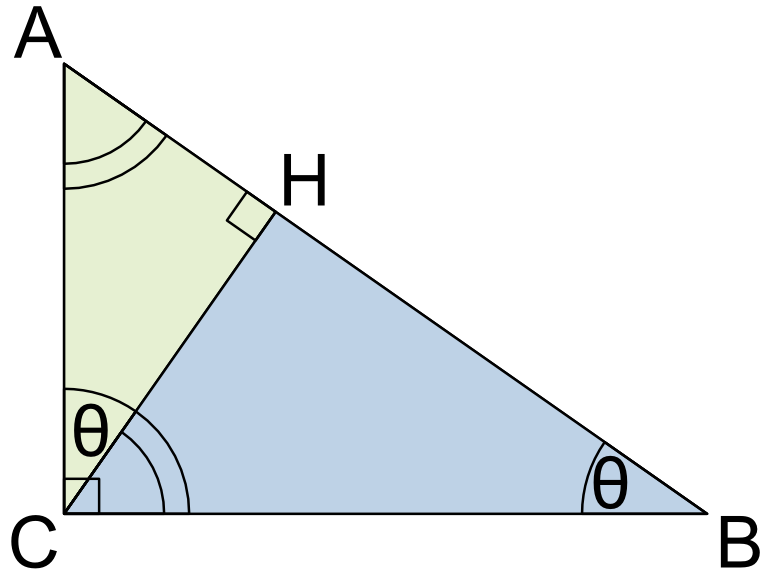
\includegraphics[width=0.3\textwidth]{figures/Pythagoras.png}
	\caption{Similar triangles used in the proof of the Pythagorean theorem.}
	\label{fig:Pythagoras}
\end{figure}

The new triangle $ACH$ is similar to triangle $ABC$, because they both have a right angle (by definition of the altitude), and they share the angle at $A$, meaning that the third angle will be the same in both triangles as well, marked as $\theta$ in Figure~\ref{fig:Pythagoras}. By a similar reasoning, the triangle $CBH$ is also similar to $ABC$. 

Similarity of the triangles leads to the equality of ratios of corresponding sides:
\begin{equation}
    \frac{BC}{AB}=\frac{BH}{BC} \text{ and } \frac{AC}{AB}=\frac{AH}{AC}.
\end{equation}
The first result equates $\cos \theta$ and the second result equates $\sin \theta$.

These ratios can be written as:
\begin{equation}
    {BC}^{2}={AB}\times {BH} \text{ and }{AC}^{2}={AB}\times {AH}.
\end{equation}
Summing these two equalities, we obtain:
\begin{equation}
    {BC}^{2}+{AC}^{2}={AB}\times {BH}+{AB}\times {AH}={AB}\times({AH}+{BH})={AB}^{2} ,
\end{equation}
which, tidying up, is the Pythagorean theorem:
\begin{equation}
    {BC}^{2}+{AC}^{2}={AB}^{2}.
\end{equation}
\end{proof}
